%%% -*-LaTeX-*-

\chapter{Background}
\label{chap:background}

In the following two sections, we will briefly review the background
on symbolic representation for natural language including
broad-coverage meaning representations and application-specific
representations. Then, we will give an overview of the linguistic
structure prediction and recent advances on deep structured
prediction.

\section[Symbolic Representations for Natural Language]{Symbolic Representations for \\Natural Language}
\label{sec:bg:symbolic}

In~\autoref{chap:intro}, we have listed several lexical, syntactic and
semantic structures in NLP. In this section, we will mainly introduce
more detailed background on the broad-coverage semantic
presentations~(\autoref{ssec:bg:broad-mr}) and application-specific
representations on dialogue~(\autoref{ssec:bg:dialogue-mr}).

Before we introduce each semantic representation, we first define the
term \kw{anchoring} and \kw{anchors}, and then we use them to organize
semantic representations in our dissertation.

\begin{itemize}
\item \textbf{Anchoring:} As the same definition of \kw{anchoring}
  used in the Meaning Representation Parsing~(MRP) shared
  task~\citep{Oep:Abe:Haj:19}, we distinguish different flavors of
  semantic graphs based on the nature of the relationship they assume
  between the linguistic surface signal~(typically a written sentence,
  i.e. a string) and the nodes of the graph. We refer to this relation
  as ~\kw{anchoring}~(of nodes onto sub-strings); other commonly used
  terms include alignment, correspondence, or lexicalization.

\item \textbf{Anchor:} We define the term~\kw{anchor} as the surface
  substring in the sentence, which is \kw{anchoring} to the
  corresponding node in the graph. According to the type of the
  substring~(lexicon, phrase, sentence, and so on), we mainly classify
  the type of the \kw{anchors} into \kw{lexical-anchoring},
  \kw{phrasal-anchoring} and \kw{sentential-anchoring}.
\end{itemize}

\subsection{Broad-coverage Semantic Representations}
\label{ssec:bg:broad-mr}

For linguistic analysis, structures have been studied from
subword-level morphology~\citep{beesley2003finite}, word-level lexicon
semantics~\citep{miller1998wordnet}, to single sentence
syntax/semantic
representations~\citep{baker1998berkeley,palmer2005proposition,collins2003head},
and multi-sentences discourse
analysis~\citep{carlson2003building,wolf2005representing,prasad2008penn}. A
broad-coverage semantic representation is a general-purpose meaning
representation language aiming to represent the multiple phenomena in
a single structure for broad-coverage text.

As shown in~\autoref{fig:intro:dog-dep}, syntactic dependency
structures capture the directed bi-lexical grammatical relations
between words. Each labeled arc represents a directed relation from
heads to dependents. However, different from the syntactic dependency
tree, semantic dependency graphs aim to represent the semantic
dependencies in the full sentence, including word sense distinctions,
the reentrances for coreference, predicate-argument structures in
semantic role labeling, named entities representations, and so
on. Because of the reentrances, semantic representations can be a
graph rather than a tree-like structure.

This dissertation covers
broad-coverage graph-based semantic representations in a single
sentence, which involves \kw{lexical-anchoring} and
\kw{phrasal-anchoring}. For lexical anchoring, we cover the DELPH-IN
MRS Bi-lexical Dependencies~\cite[DM,][]{ivanova2012did} and Prague
Semantic
Dependencies~\cite[PSD,][]{hajic2012announcing,miyao2014house},
Abstract Meaning Representation~\cite[AMR,][]{Ban:Bon:Cai:13}; While
for phrasal-anchoring, we study Universal Conceptual Cognitive
Annotation~\cite[UCCA,][]{Abe:Rap:13b}. We consider a famous
sentence~(\#20001001 in MRP Corpus) as a running example, which is
also the first sentence from WallStreetJournal~(WSJ) Corpus from the
Penn Treebank~\citep{Mar:San:Mar:93}: \emph{\dquoted{Pierre Vinken, 61
    years old, will join the board as a nonexecutive director
    Nov.29.}} This sentence contains some interesting linguistic
phenomes, such as morphology words, person, and date named
entities. Taking it as an example, we will introduce the detailed
properties for each of the representations.~\footnote{The
  summarization paper in MRP workshop~\citep{Mar:San:Mar:93}
  introduces another example-based comparative studies for different
  meaning representations.}

%\subsubsection{Bi-lexical Semantic Dependencies}
%\label{ssec:bg:bi-leixcal}

\subsubsection{DELPH-IN MRS-Derived Bi-lexical Dependencies}
\label{sssec:bg:dm}

\begin{figure}[!th]
\centering
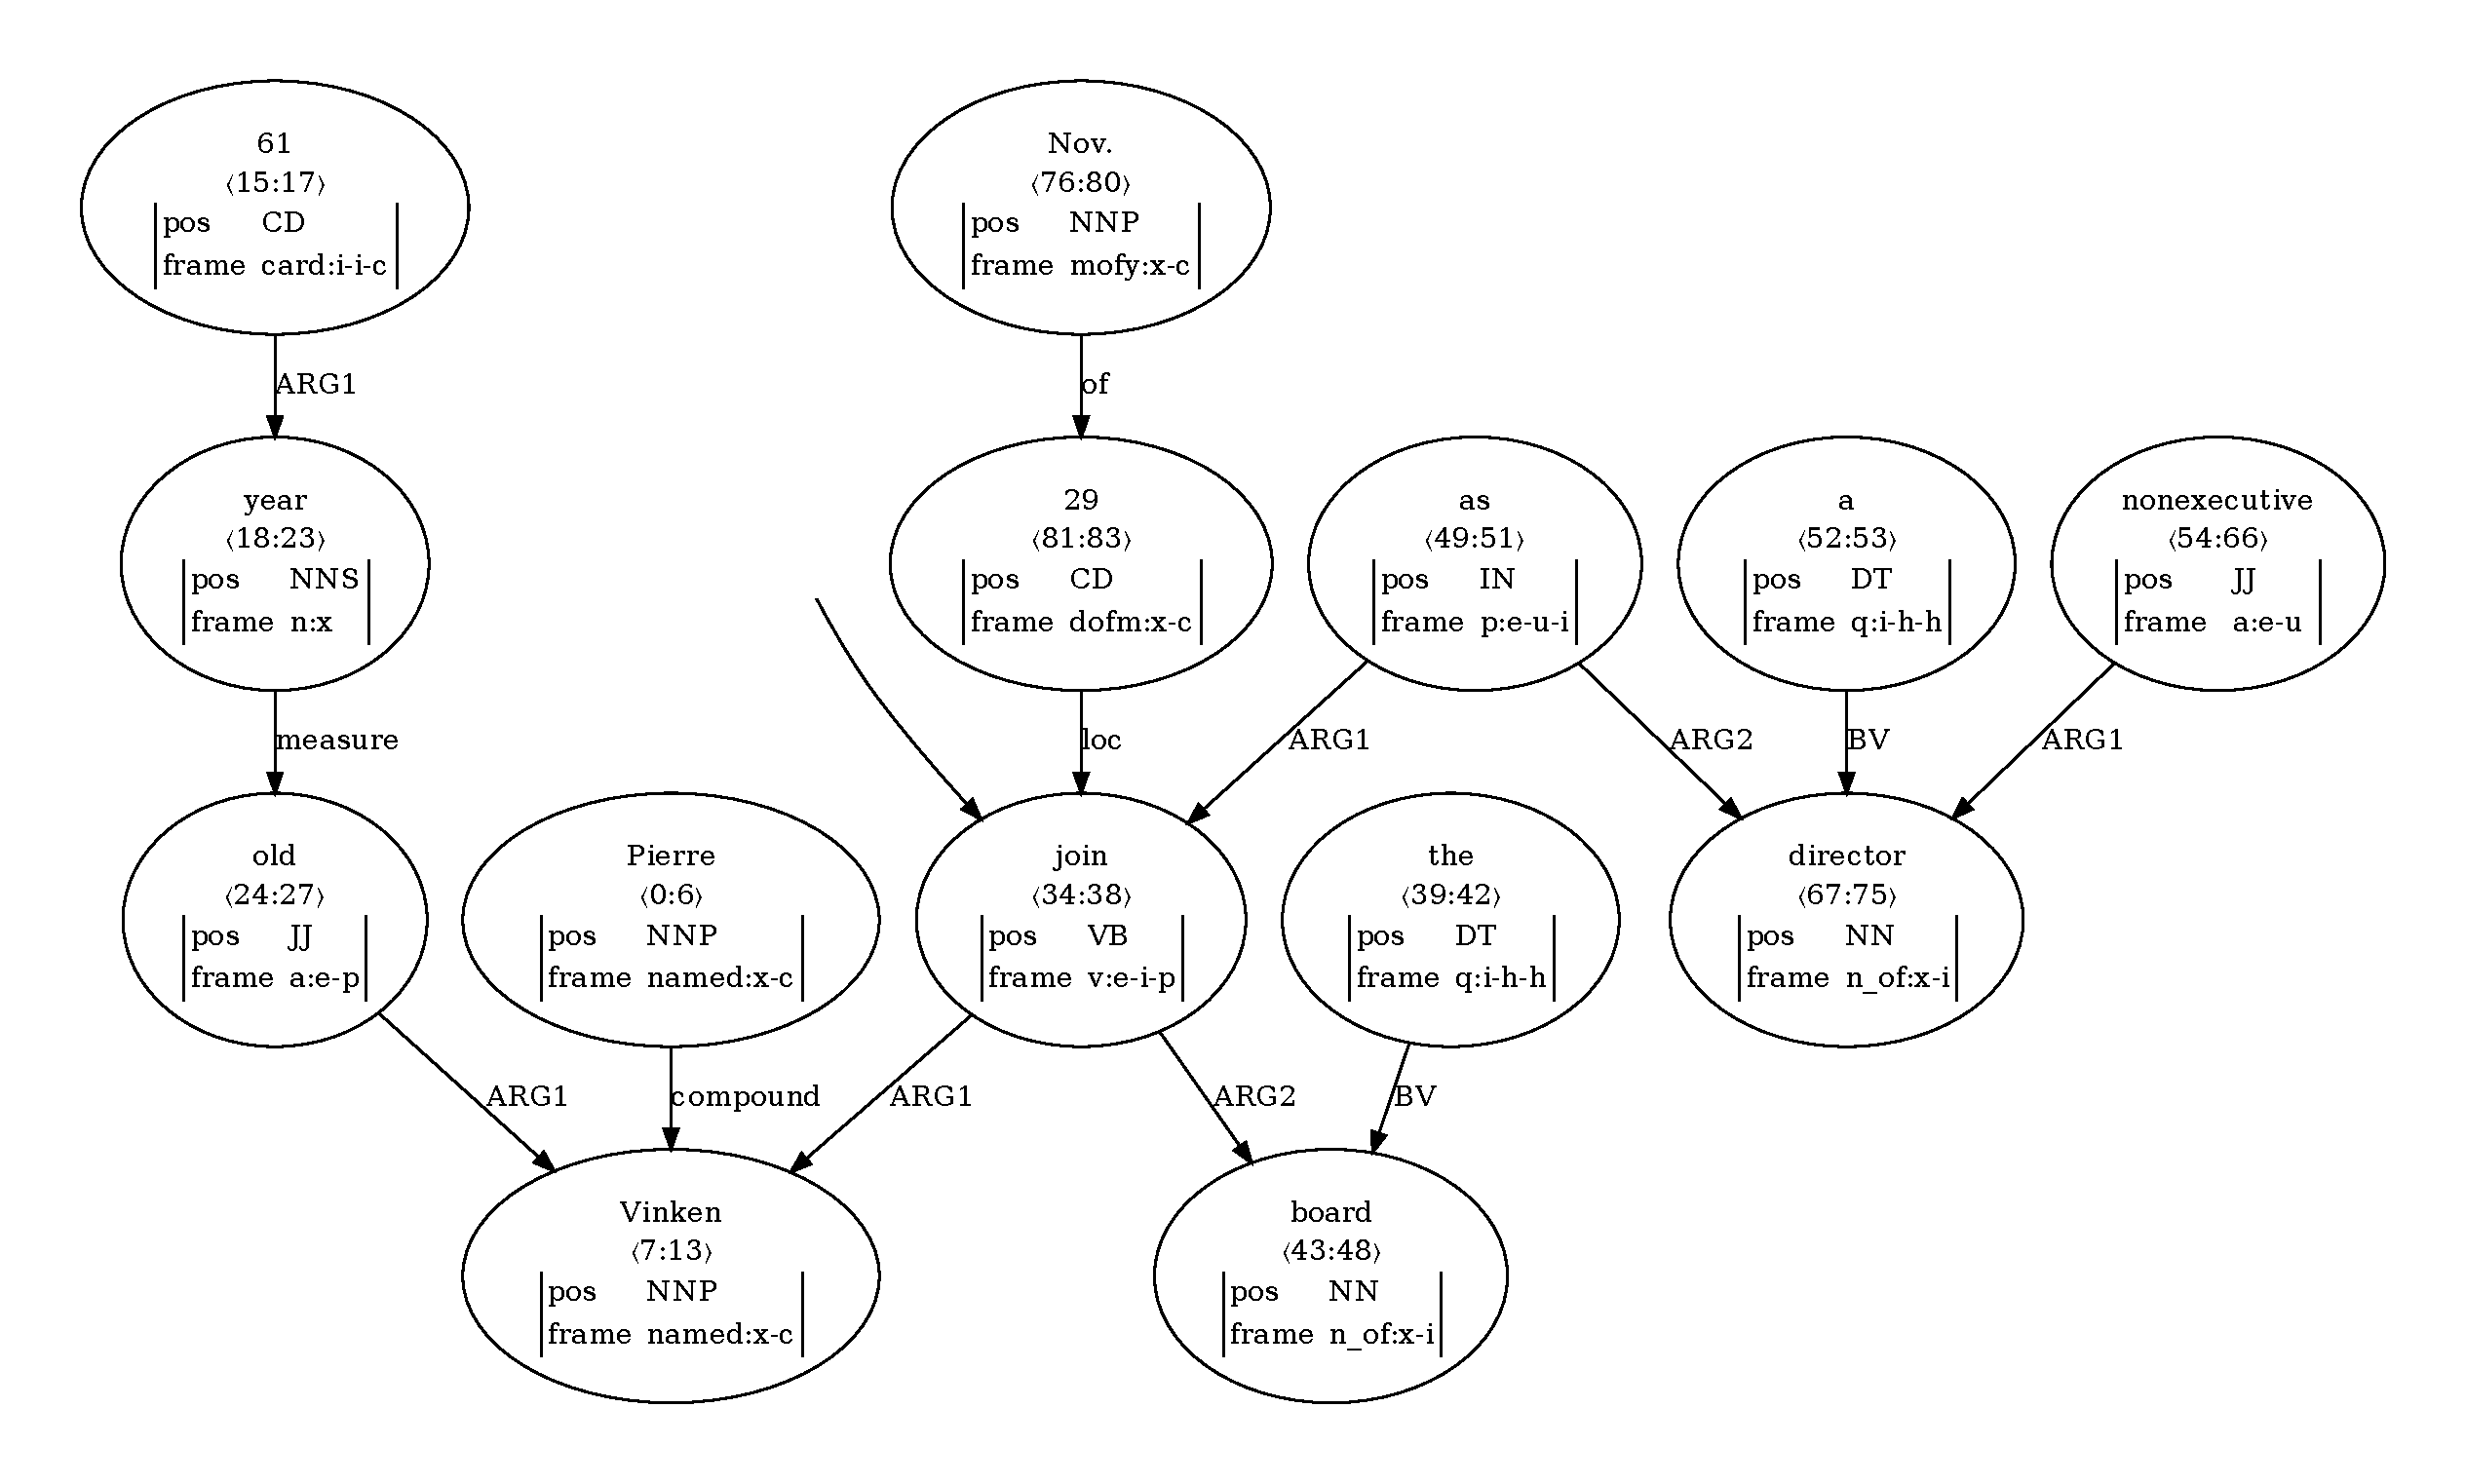
\includegraphics[width=0.90\textwidth]{bg/dm-20001001.pdf}
\caption{\label{fig:bg:dm}The DM representation for the sentence
  \#20001001}
\end{figure}

It originates in a manual reannotation, dubbed
DeepBank~\citep{Fli:Kor:Zha:12}, with syntactic-semantic analyses of
the LinGO English Resource Grammar~\citep{Oep:Fli:Tou:04} in logical
forms. These logical forms are often referred to as English Resource
Semantics~\citep[ERS,][]{Ben:Fli:Oep:15}, and the underlying grammar
is rooted in the general linguistic theory of Head-Driven Phrase
Structure Grammar~\citep[HPSG,][]{Pol:Sag:94}. Then
\citet{Iva:Oep:Ovr:12} propose a two-stage version to transform the
ERS logical forms into bi-lexical semantic dependency graphs. ERS
logical forms are firstly transformed into Elementary Dependency
Structures~\citep[EDS,][]{Oep:Lon:06}, then EDS are simplified into
pure bi-lexical dependencies, dubbed DELPH-IN MRS Bi-Lexical
Dependencies~\citep[DM,][]{Iva:Oep:Ovr:12}. As shown
in~\autoref{fig:bg:dm}, graph nodes in DM are anchoring to the surface
tokens. Hence, DM is lexical-anchoring. However, the underlying tokens
are not fully covered in the graph. For example, the word
\tquoted{will} does not produce any node in the DM graph. Edges mainly
indicate semantic argument roles~(ARG1, ARG2, ...) into the relation
corresponding to their source node~\footnote{The annotation of
  predicate-argument structures is based on the semantic
  inferface~(SEM-I) in the ERG. Please refer to this introduction for
  more
  details.\url{https://github.com/delph-in/docs/wiki/ErgSemantics_Interface}},
but there are some more specialized edge labels too. For example, it
uses \kw{compound} to reflect the name~\tquoted{Pierre Vinken} as a
whole, and it uses BV (bound variable, e.g., the word \tquoted{a}) as
a reflection of quantification in the underlying logic
quantification. In summary, DM is lexical-anchoring, and it captures
semantic phenomena including predicate-argument structures, word-sense
differentiation, quantification, and scope.

\begin{figure}[!th]
\centering
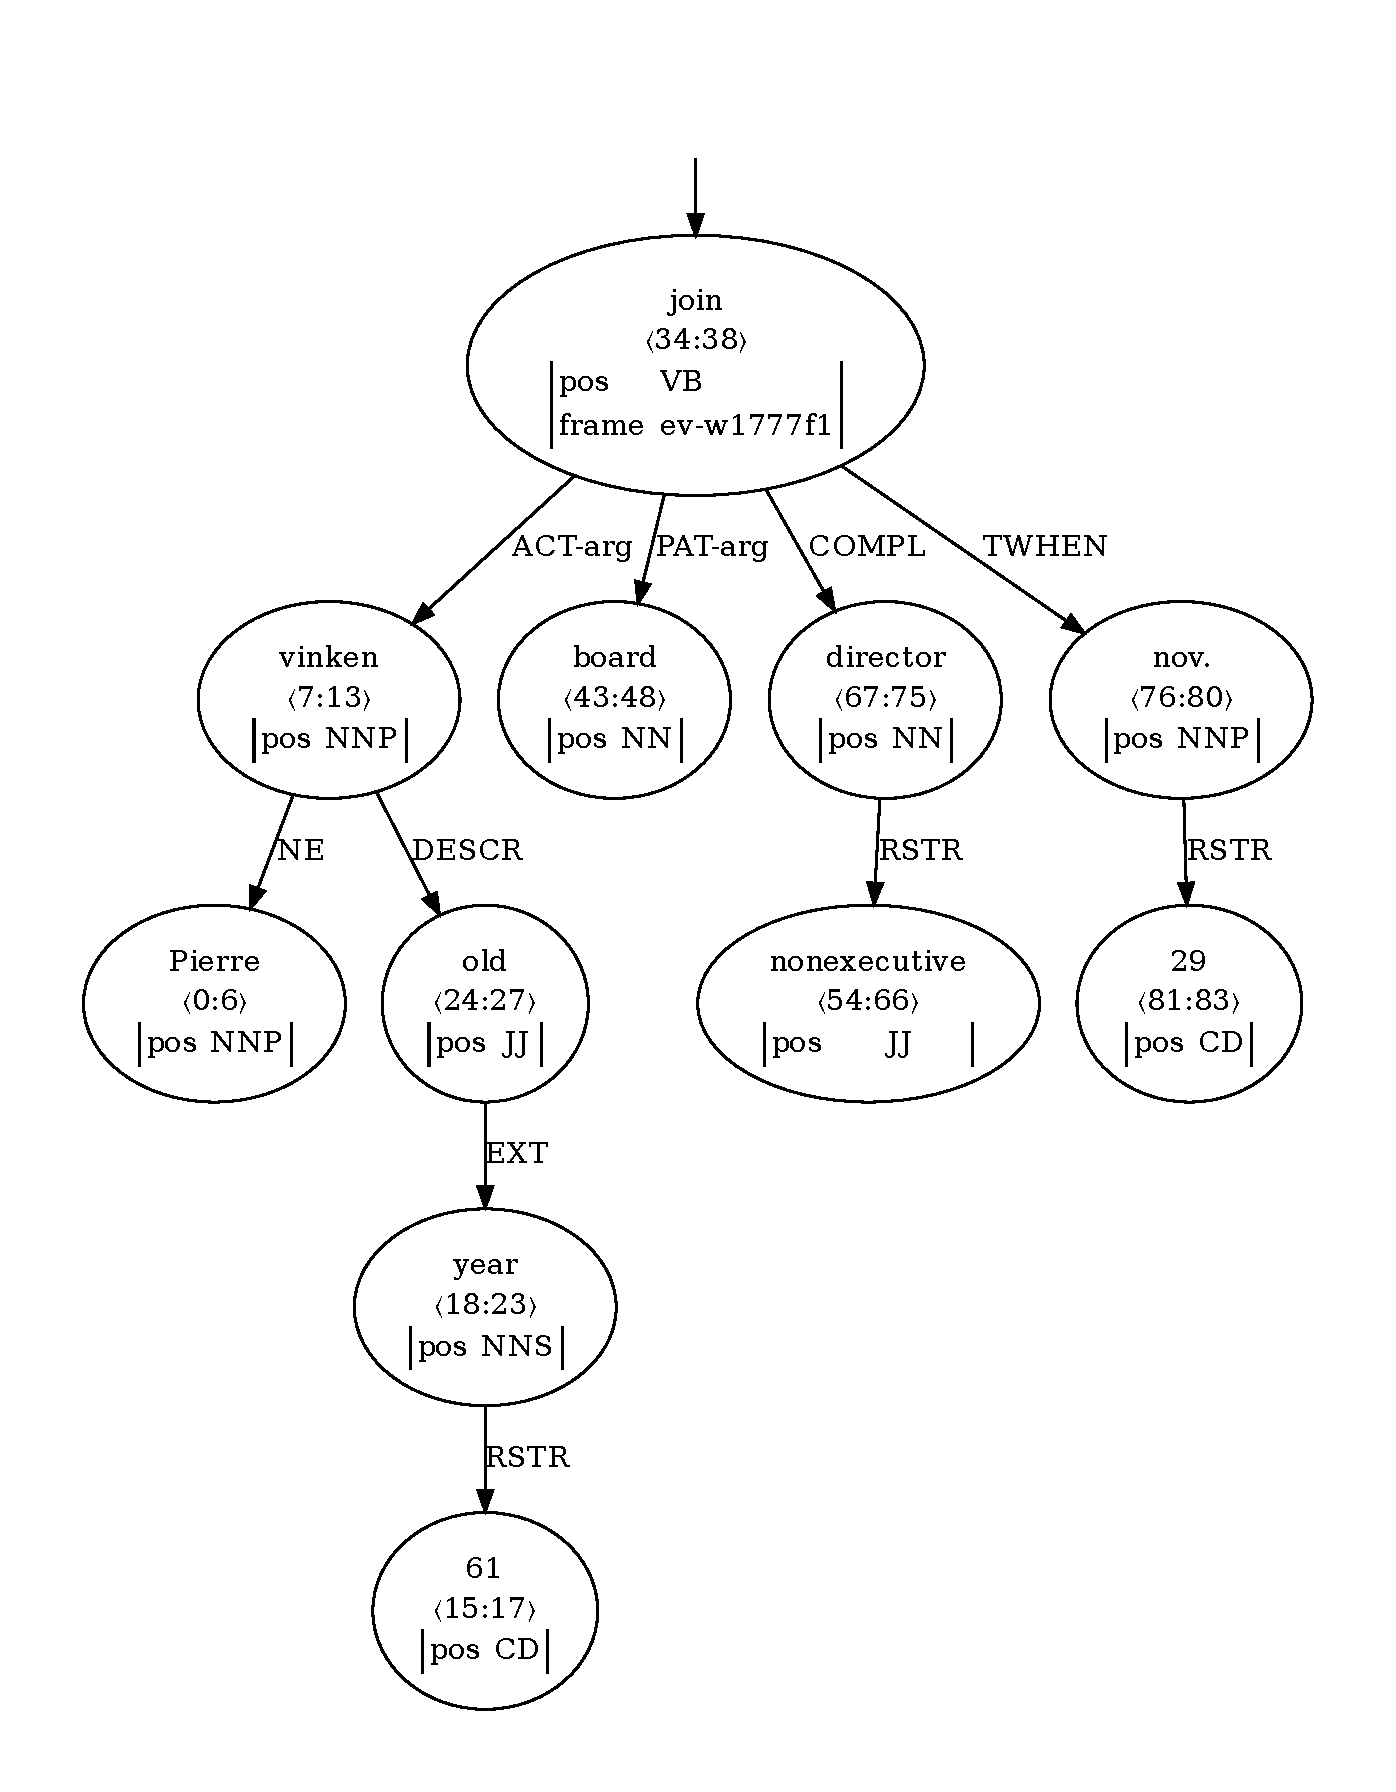
\includegraphics[width=0.98\textwidth]{bg/psd-20001001.pdf}
\caption{\label{fig:bg:psd}The PSD representation for the sentence
  \#20001001}
\end{figure}

\subsubsection{Prague Semantic Dependencies}
\label{sssec:bg:psd}
Besides DM, there is another line of research to simplify the richer
syntactic-semantic representations into bi-lexical semantic
dependencies. It adopts the reduction of tectogrammatical trees (or
t-trees) from the linguistic school of Functional Generative
Description~\citep[FGD,][]{Sga:Haj:Pan:86,hajic2012announcing} into
PSD. The Prague Czech-English Dependency
Treebank~\citep[PCEDT,][]{hajic2012announcing} is a set of parallel
dependency trees over the WSJ texts from the PTB and their Czech
translations. The PSD bi-lexical dependencies are extracted from the
tectogrammatical annotation layer. Top nodes are derived from t-tree
roots; Especially, they mostly correspond to main verbs. In the case
of coordinate clauses, there are multiple top nodes per
sentence. \autoref{fig:bg:psd} shows the PSD representation of our
example sentence. One major differences are the role labels and verb
frames, they are grounded in a machine-readable valency
lexicon~\citep{urevsova2016czengvallex}, and the frame values on
verbal nodes indicate specific verbal senses in the
lexicon. In a summary, PSD is also lexical-anchoring, and it
  captures the same semantic contents with DM~(including
  predicate-argument structures, word-sense, quantification and
  scope), however, with a different formation and different frame
  lexicon.

%\begin{figure}[!th]
%  \centering
%  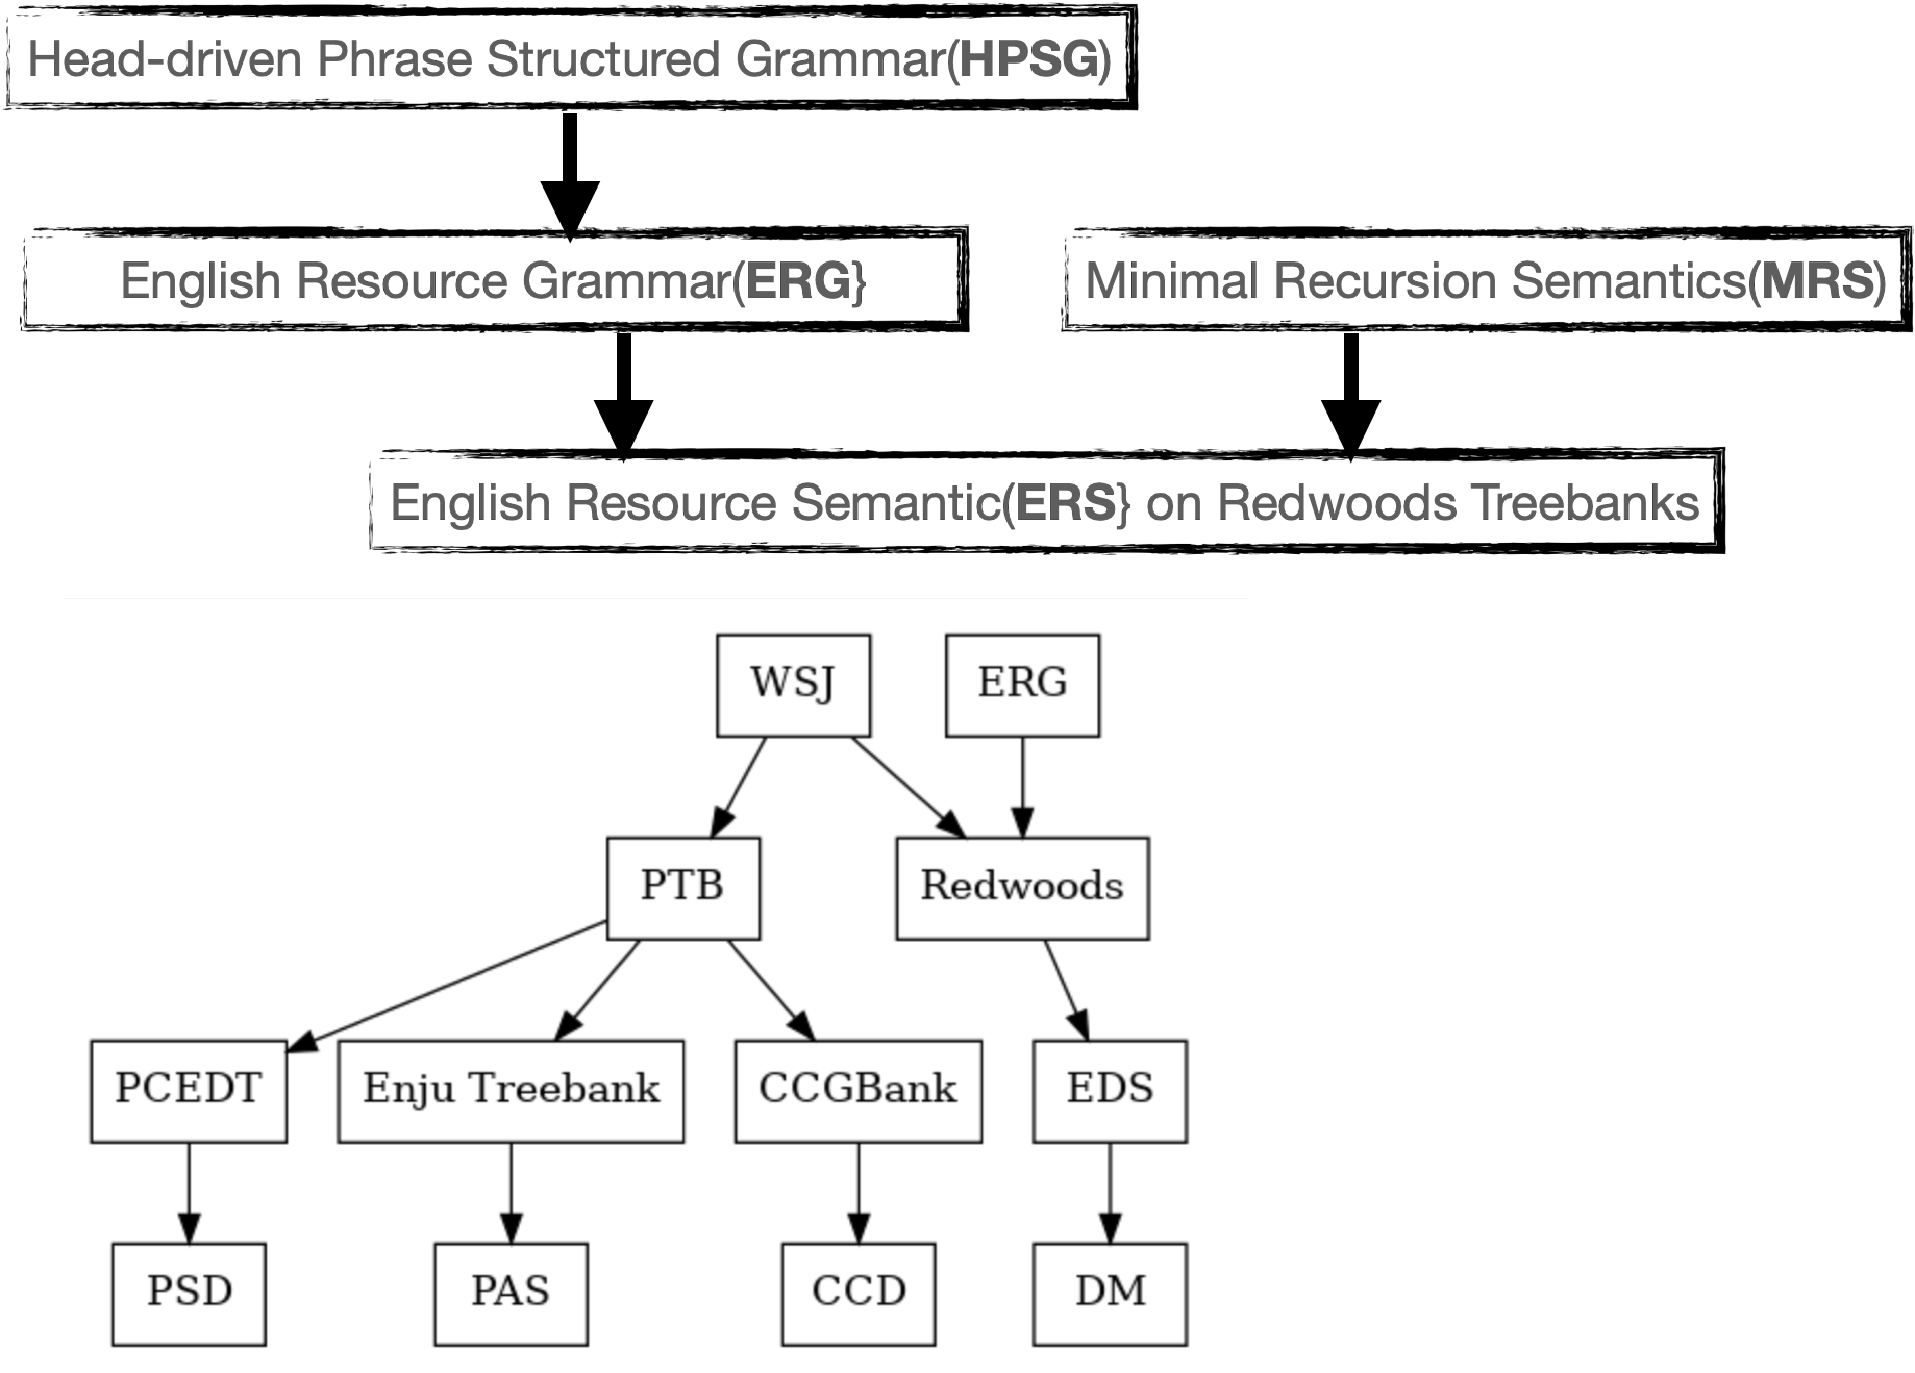
\includegraphics[width=0.98\textwidth]{bg/dm-psd-history.pdf}
%\caption{\label{fig:dm-psd-history}The hierarchical relations between
%  DM, PSD, and their underlying grammar and semantics}
%\end{figure}


\subsubsection{Abstract Meaning Representation}
\label{ssec:bg:amr}
%
\begin{figure}[!th]
\centering
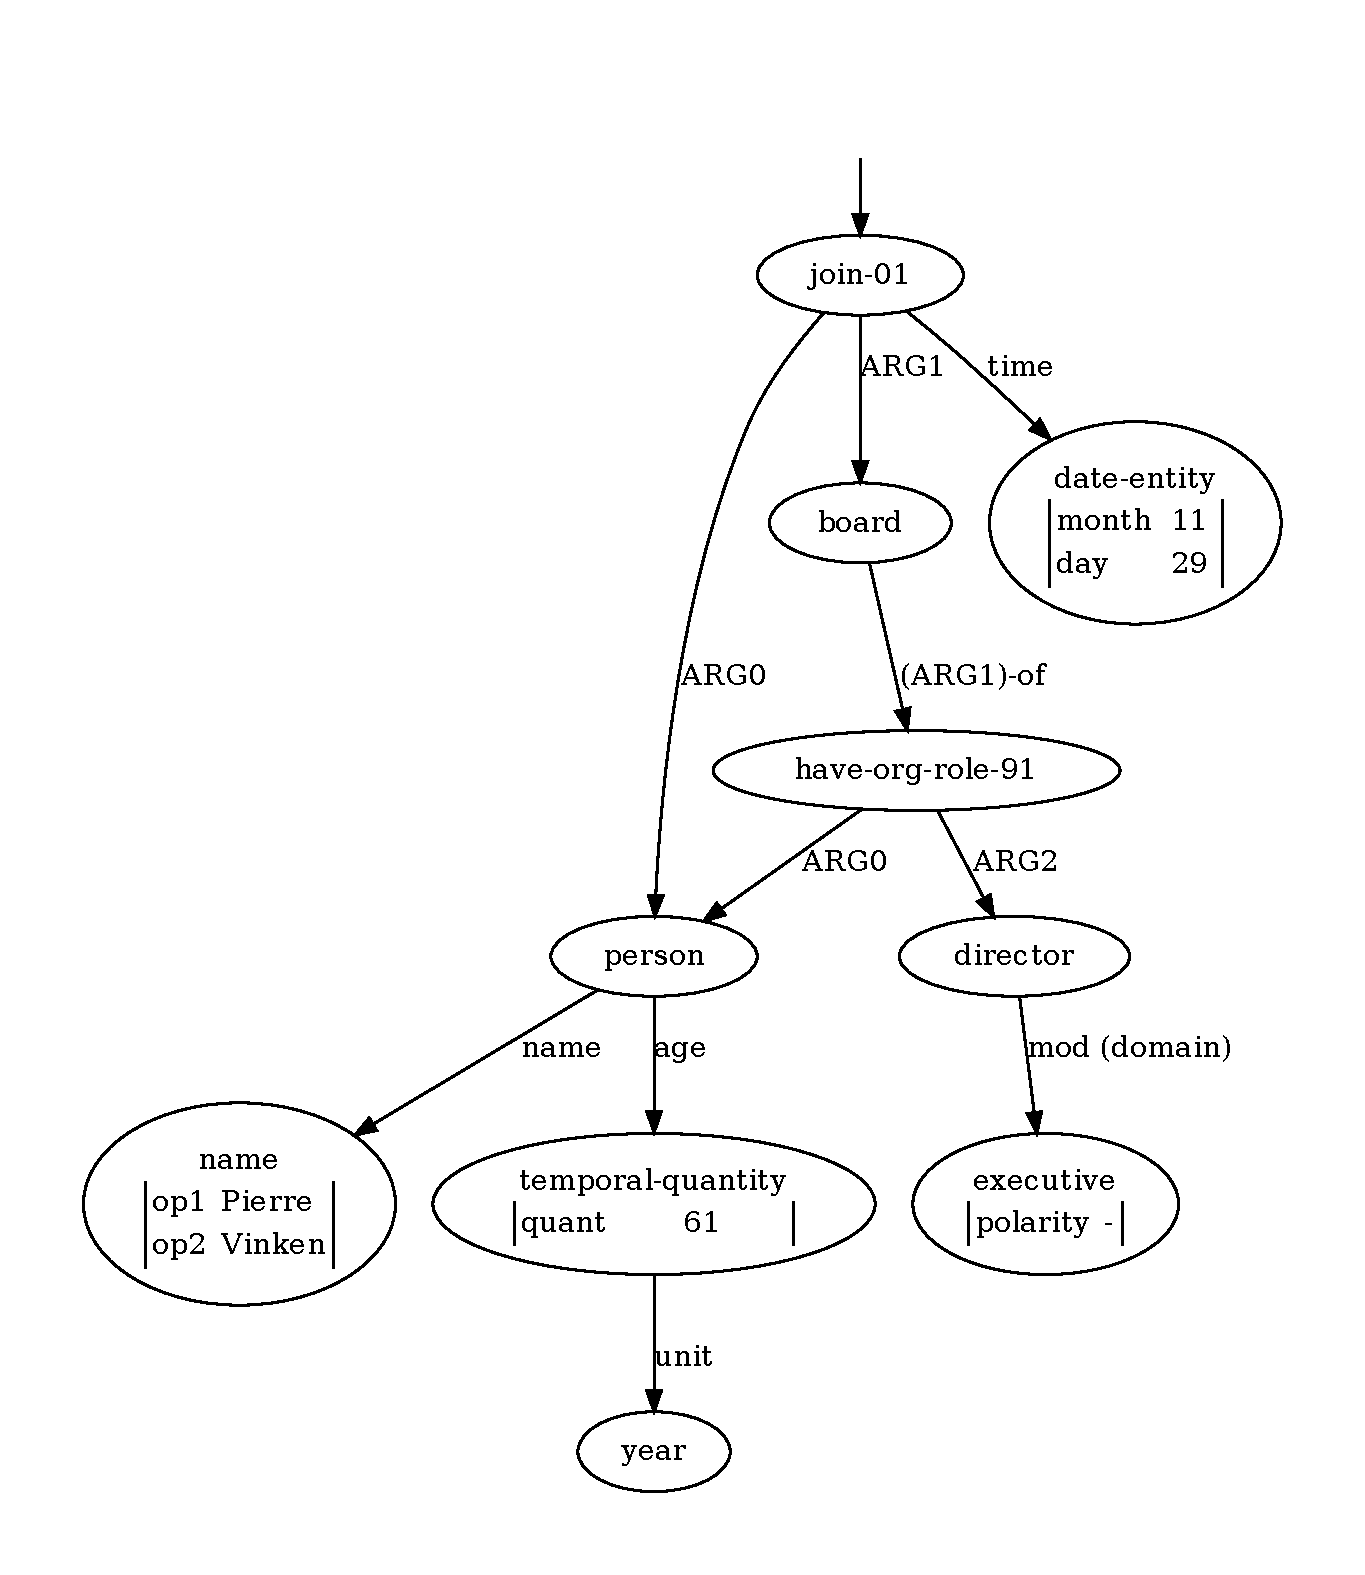
\includegraphics[width=0.98\textwidth]{bg/amr-20001001.pdf}
\caption{\label{fig:bg:amr} The AMR representation for the sentence
  \#20001001}
\end{figure}

As shown in~\autoref{fig:bg:amr}, Abstract Meaning Representation
represents sentence meaning as directed graphs with labeled nodes
~(concepts) and edges~(relations). AMRs are rooted, labeled graphs
that are easy for people to read and easy for programs to traverse.
AMR concepts are either English words (\tquoted{board}), PropBank
framesets (\tquoted{join-01}), or special entity
keywords~(\tquoted{date-entity}, \tquoted{person}, \tquoted{name},
etc.), quantities~(\tquoted{temporal-quantity},
\tquoted{distance-quantity}, etc.), and logical
conjunctions~(\tquoted{and}, etc).  AMR strives for a more logical,
less syntactic representation. For example, it represents the
word~\tquoted{nonexecutive} with a negation~\tquoted{(:polarity 0)}
with the concept~\tquoted{executive}. Furthermore, unlike DM and PSD
on predicate-argument representation, AMR extensively uses PropBank
framesets~\citep{Kin:Pal:02, palmer2005proposition}. For example, It
represents the verb~\tquoted{join} using the
frame~\tquoted{join-01}. At the meantime, AMR also newly designs
special frames to reuse those core roles in Propbank. As shown in
~\autoref{fig:bg:amr}, the word~\tquoted{board} have a role
\tquoted{ARG1-of} to a special frame~\tquoted{have-org-role-91}.

The above abstraction allows for concepts and relations not explicitly
mentioned in the text but leaves open the question of how these are
derived from the text. This question is important because training
statistical AMR parsers typically start with a conjectured alignment
between tokens and the graph elements. Most AMR
parsers~\cite[\eg][]{Flanigan:2014vc,Wang:2015uo,Artzi:2009tb,Pust:2015ug,Peng:2015tj,Konstas:2017uj,Wang:2017vt}
use either the JAMR aligner~\cite{Flanigan:2014vc} or the ISI
aligner~\cite{Pourdamghani:2014aligning} for this
purpose\footnote{Other aligners exist, \eg
  \citet{chen2017unsupervised} uses dependencies, but raw text
  alignments are more prevalent.}  We introduced more details about
AMR alignment in~\autoref{ssec:lex-phr:amr-anchor}, and we show that
AMR nodes and subgraphs are implicitly anchored to the lexical tokens
or entities. In summary, AMR is implicit lexical-anchorin, and it
captures more semantic content than DM and PSD. Besides the common
predicate-argument structure, word sense, qutification, and scope~(by
placing~\tquoted{polarity}), AMR also represents the lexical
decomposion, anaphoric coreference, and entity-linking.

\subsubsection{Universal Conceptual Cognitive Anotation}
\label{ssec:bg:ucca}

\begin{figure}[!th]
\centering
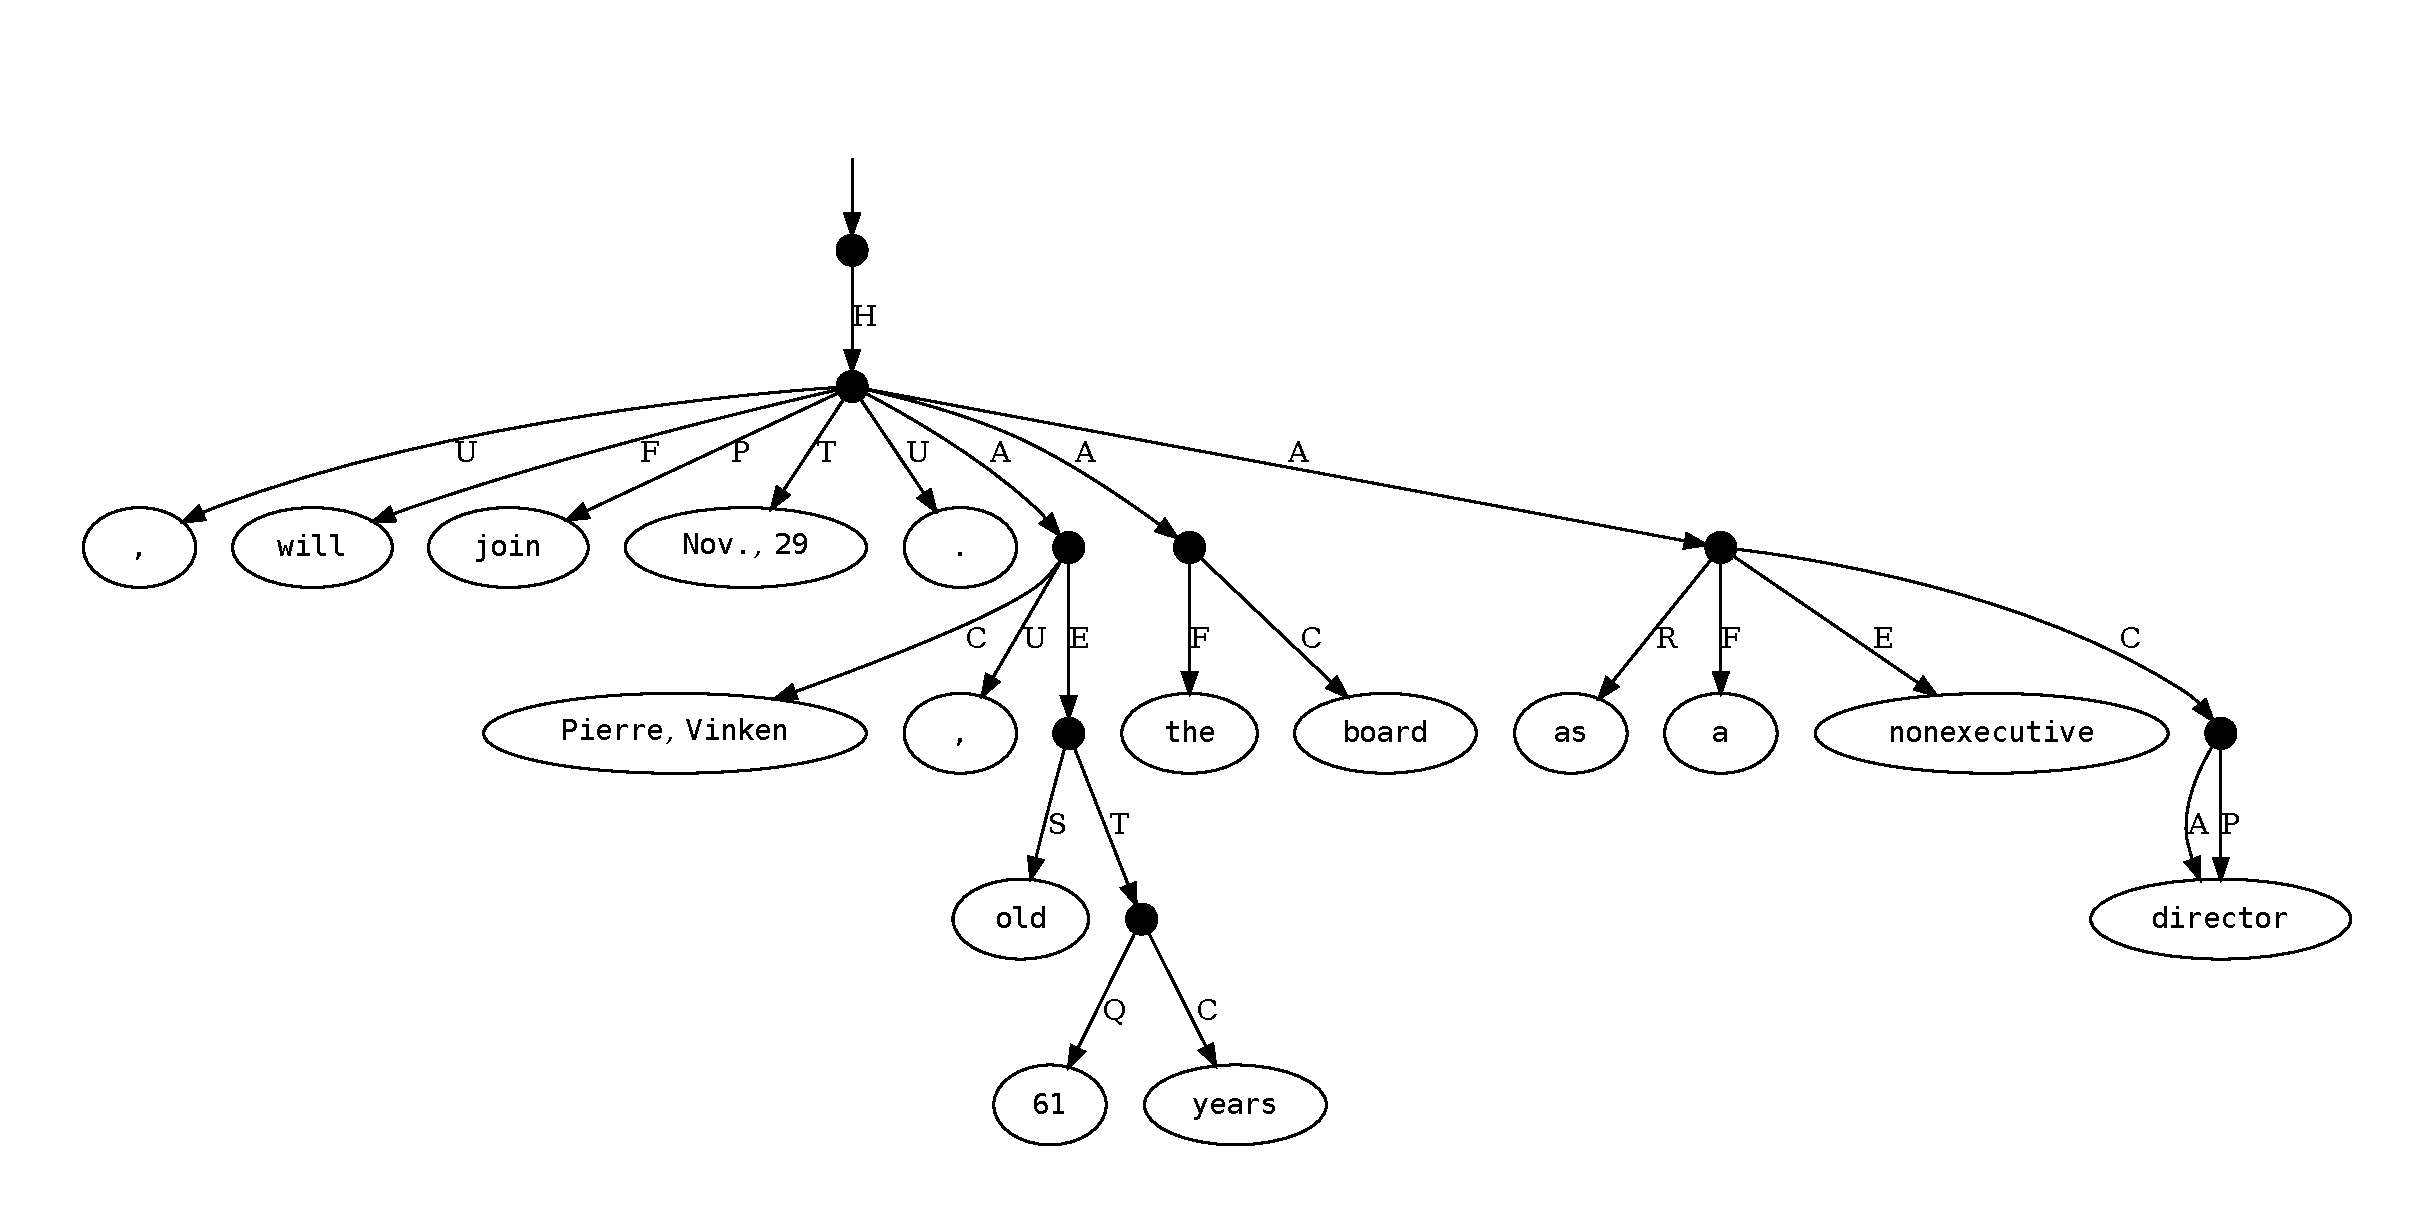
\includegraphics[width=0.99\textwidth]{bg/ucca-20001001.pdf}
\caption{\label{fig:bg:ucca}The UCCA representation for the sentence
  \#20001001}
\end{figure}

Similar to AMR, UCCA is designed to abstract the semantic scheme away
from its surface and syntactic forms. UCCA uses directed acyclic
graphs~(DAGs) to represent its semantic structures. The atomic
meaning-bearing units are placed at the leaves of the DAG and are
called terminals. The nodes of the graph are called units. A unit may
be either~(i)~a terminal or~(ii)~several elements jointly viewed as a
single entity according to some semantic or cognitive
consideration. In many cases, a non-terminal unit is comprised of a
single relation and the units it applies to (its arguments). In some
cases it may also contain secondary relations. Hierarchy is formed by
using units as arguments or relations in other units.

While different from previous DM, PSD, and AMR, categories are not
annotated on nodes, but edges and represent the descendant unit's role
in forming the semantics of the parent unit. The foundational layer
covers the entire text, so each word participates in at least one
unit. It focuses on argument structures of verbal, nominal, and
adjectival predicates and the inter-relations between them. Argument
structure phenomena are considered fundamental by many approaches to
semantic and grammatical representation and have a high applicative
value, as demonstrated by their extensive use in NLP. The foundational
layer views the text as a collection of Scenes. A Scene can describe
some movement or action or a temporally persistent state. As shown
in~\autoref{fig:bg:ucca}, for the event~\tquoted{join the board},
~\tquoted{join} with an incoming edge~\tquoted{P} denoting the
category~\tquoted{Process}, which is the primary relation of a scene
that evolves in time. While the edge~\tquoted{A} linked to the
non-terminal node corresponding to~\tquoted{Pierre, Vinken, 61 years
  old} means the unit~\tquoted{Pierre, Vinken} is the participant of
the scene. In sum, UCCA is phrasal-anchoring, and its foundational
layer captures predicate-argument structures, anaphoric coreference,
representing less semantic content than DM, PSD, and AMR. However,
UCCA shows more benefits on cross-lingual, easy annotation, and
extensible modularity.

\subsubsection{Summary}
\label{ssec:bg:summary-broad-coverage}

For easy reference, in~\autoref{tbl:bg:summary-broad-coverage}, we
summarize the background of broad-coverage meaning representations for
the their anchoring type and captured semantic phenomena. For more
detailed comparative studies over the state-of-art semantic
representation, please refer to the paper~\citep{abend2017state}.

\begin{table}[ht]
\caption{The summary of broad-coverage meaning representation, with respect to their anchoring type and captured semantic contents}
  \begin{center}
\setlength{\tabcolsep}{4pt}
{
\begin{tabular}{c|cccc}
  \toprule
  \hline
  & {\bf DM}               & {\bf PSD}              & {\bf AMR}              & {\bf UCCA}    \\ \hline
  Anchoring Type          & Explicit Lexical & Explicit Lexical & Implicit Lexical & Phrasal \\ \hline
  Predicate-Argument      & Yes              & Yes              & Yes              & Yes     \\
  Word Sense              & Yes              & Yes              & Yes              & No      \\
  Qualification and Scope & Partial          & No               & Yes              & No      \\
  Presupposition/Focus    & No               & No               & Yes              & No      \\
  Lexical Decomposition   & No               & No               & Yes              & No      \\
  Anaphoric Coreference   & No               & No               & Partial          & Partial \\
  Grounding               & No               & No               & Yes              & No \\ \hline
  \bottomrule

\end{tabular}}
\end{center}
\label{tbl:bg:summary-broad-coverage}
\end{table}


\subsection{Application-specific Representation on Dialogue}
\label{ssec:bg:dialogue-mr}

In this dissertation, we ground the study on application-specific
representation on dialogue. The following section will introduce the
dialog representations via dialogue act, dialog state, and richer
conversational semantic representations.

\subsubsection{Dialogue Act and MISC Codes}
\label{sssec:bg:dialogue-act}
In the utterance-level, dialogue acts are designed to represent the
function of each utterance in the dialogue. The key insight behind the
dialogue act is that each utterance in a dialogue is a kind of action
being performed by the speaker. The history of dialogue act can be
derived back to the philosopher~\citet{wittgenstein2010philosophical}.
A dialogue act has two main components: a communicative function and a
semantic content. \citet{bunt2010towards} provides an ISO project
developing an international standard for annotating dialogue with
semantic information, particularly concerning the communicative
functions of the utterances, the kind of content they address, and the
dependency relations to what was said and done earlier in the
dialogue. Similarly, Motivational Interview Skill Codes
~\cite[MISC,][]{miller2003motivational,miller2012motivational} are
also proposed to represent the functions of each client and therapist
utterance in the psychotherapy dialogue. This part will mainly
introduce the MISC Codes for psychotherapy dialogue.

%% putting the table here to make it in the second page.
\begin{table}[ht]
\caption{Distribution, description and examples of MISC labels.}
  \begin{center}
\setlength{\tabcolsep}{4pt}
{\small
\begin{tabular}{llll}
  \toprule
  {\bf Code}            & {\bf Count}            & {\bf Description}                                                                                            & {\bf Examples}                                    \\
  \midrule \midrule
  \multicolumn{4}{c}{ \bf Client Behavioral Codes }                                                                                                                                                                 \\
  \midrule
  \multirow{2}{*}{\FN}  & \multirow{2}{*}{47715} & \multirow{2}{*}{\parbox{5.5cm}{Follow/ Neutral: unrelated to changing or sustaining behavior.}}              & ``You know, I didn't smoke for a while.''         \\
                        &                        &                                                                                                              & ``I have smoked for forty years now.''            \\
  \CHANGE               & \multirow{2}{*}{5099}  & \multirow{2}{*}{\parbox{5.5cm}{Utterances about changing unhealthy  behavior.}}                                                                          & ``I want to stop smoking.''                       \\
                        & \\
  \SUSTAIN              & \multirow{2}{*}{4378}  & \multirow{2}{*}{\parbox{5.5cm}{Utterances about sustaining unhealthy behavior.}}                                                                        & ``I really don't think I smoke too much.''        \\
                        & \\ \midrule
  \midrule
  \multicolumn{4}{c}{\bf Therapist Behavioral Codes }                                                                                                                                                               \\
  \midrule
  \FA                   & 17468                  & Facilitate conversation                                                                                      & ``Mm Hmm.'', ``OK.'',``Tell me more.''            \\
  \GI                   & 15271                  & Give information or feedback.                                                                                & ``I'm Steve.'', ``Yes, alcohol is a depressant.'' \\
  \multirow{2}{*}{\RES} & \multirow{2}{*}{6246}  & \multirow{2}{*}{\parbox{5.5cm}{Simple reflection about the client's most recent utterance.}}                 & C: ``I didn't smoke last week''                   \\
                        &                        &                                                                                                              & T: ``Cool, you avoided smoking last week.''       \\
  \multirow{2}{*}{\REC} & \multirow{2}{*}{4651}  & \multirow{2}{*}{\parbox{5.5cm}{Complex reflection based on a client's conversation history.}} & C: ``I didn't smoke last week.''                  \\
                        &                        &                                                                                                              & T: ``You mean things begin to change''.           \\
  \QUC                  & 5218                   & Closed question                                                                                              & ``Did you smoke this week?''                      \\
  \QUO                  & 4509                   & Open question                                                                                                & ``Tell me more about your week.''                 \\
  \multirow{2}{*}{\MIA} & \multirow{2}{*}{3869}  & \multirow{2}{*}{\parbox{5.5cm}{MI adherent,~\eg, affirmation, advising with permission, etc.}}          & ``You've accomplished a difficult task.''         \\
                        &                        &                                                                                                              & ``Is it OK if I suggested something?''            \\
  \multirow{2}{*}{\MIN} & \multirow{2}{*}{1019}  & \multirow{2}{*}{\parbox{5.5cm}{MI non-adherent,~\eg, confront, advising without permission, etc.}}      & ``You hurt the baby's health for cigarettes?''    \\
                        &                        &                                                                                                              & ``You ask them not to drink at your house.''      \\\bottomrule
\end{tabular}}
\end{center}
\label{tbl:bg:misc}
\end{table}

Motivational Interviewing~(MI) is a style of psychotherapy that seeks
to resolve a client's ambivalence towards their problems, thereby
motivating behavior change. Several meta-analyses and empirical
studies have shown MI's high efficacy and success in
psychotherapy~\citep{burke2004emerging, martins2009review,
  lundahl2010meta}. However, MI skills take practice to master and
require ongoing coaching and feedback to sustain~\citep{Schwalbe2014}.
Given the emphasis on using specific types of linguistic behaviors in
MI~(\eg, open questions and reflections), fine-grained behavioral
coding plays an essential role in MI theory and training.

Motivational Interviewing Skill Codes~(MISC, ~\autoref{tbl:bg:misc})
is a framework for coding MI sessions. It facilitates evaluating
therapy sessions via utterance-level labels akin to dialogue
acts~\citep{stolcke2000dialogue,jurafsky2018speech}, and are designed
to examine therapist and client behavior in a therapy
session.\footnote{The original MISC description of
  \citet{miller2003manual} included 28 labels (9 client, 19
  therapist). Due to data scarcity and label confusion, various
  strategies are proposed to merge the labels into a coarser set.  We
  adopt the grouping proposed by~\citet{xiao2016behavioral};
  ~\autoref{ssec:misc_clustering} gives more details.}
\autoref{tbl:bg:misc} shows the distribution, description and examples
of MISC labels for clients and therapists. Each of the MISC labels
will be corresponding to a single utterance. Hence, MISC code
prediction is a sentence-anchoring task, mainly capturing each
utterance's function.

\subsubsection{Dialog State Tracking}
\label{ssec:bg:dialogue-state}
From the simple GUS~\citep{bobrow1977gus} to the modern task-based
dialogue systems built in virtual assistants~(Alexa, Siri, and Google
Assistant~\etal), they are all based around frames. Frame theory is
derived from Fillmore's case theory~\citep{Fillmore:68}. A frame is a
kind of knowledge structure representing the kinds of intentions the
system can extract from user sentences and consists of a collection of
slots, each of which can take a set of possible values. Together this
set of frames is sometimes called a domain ontology.

As the dialogue goes on, a dialogue state tracker maintains the
current state of the conversation (which includes the user's most recent
dialogue intent, plus the entire set of slot-filler constraints the
user has expressed so far). The dialogue policy decides what the
system should do or say next. Finally, dialogue state systems have a
natural language generation component to reply to the utterance of users.

\autoref{fig:intro:dialogue} shows a dialogue on restaurant booking
service. For each user turn, the dialogue state tracking predicts the
corresponding intent, requested slot, and slot values for that
turn. The intent classification task is to understand what the user is
trying to accomplish in this dialogue utterance; thus, the output
intent label is anchored to the current user utterance. The requested
slot is what the user is asking for more information, while the slot
filling task is to extract the particular slots and fillers that the
user offered to the system for more detailed arguments of their
intent. The requested slots and slot-filling tasks can depend on any
relevant tokens or phrases in the user utterance; thus, the anchoring
is mixed.

\subsubsection{Conversational Semantic Representations}
\label{ssec:bg:dialogue-rep}
Most existing annotations for task-oriented dialog systems have fallen
on the extremes of non-recursive intent and slot tagging, such as in
the MultiWOZ~\citep{budzianowski2018multiwoz}. Hence, the previous
intent-slot dialog state representation has poor compositionality to
represent complex conversational requests, such multiple intents in the
same utterance, and nested intent slot structures.

\begin{figure}[!th]
\centering
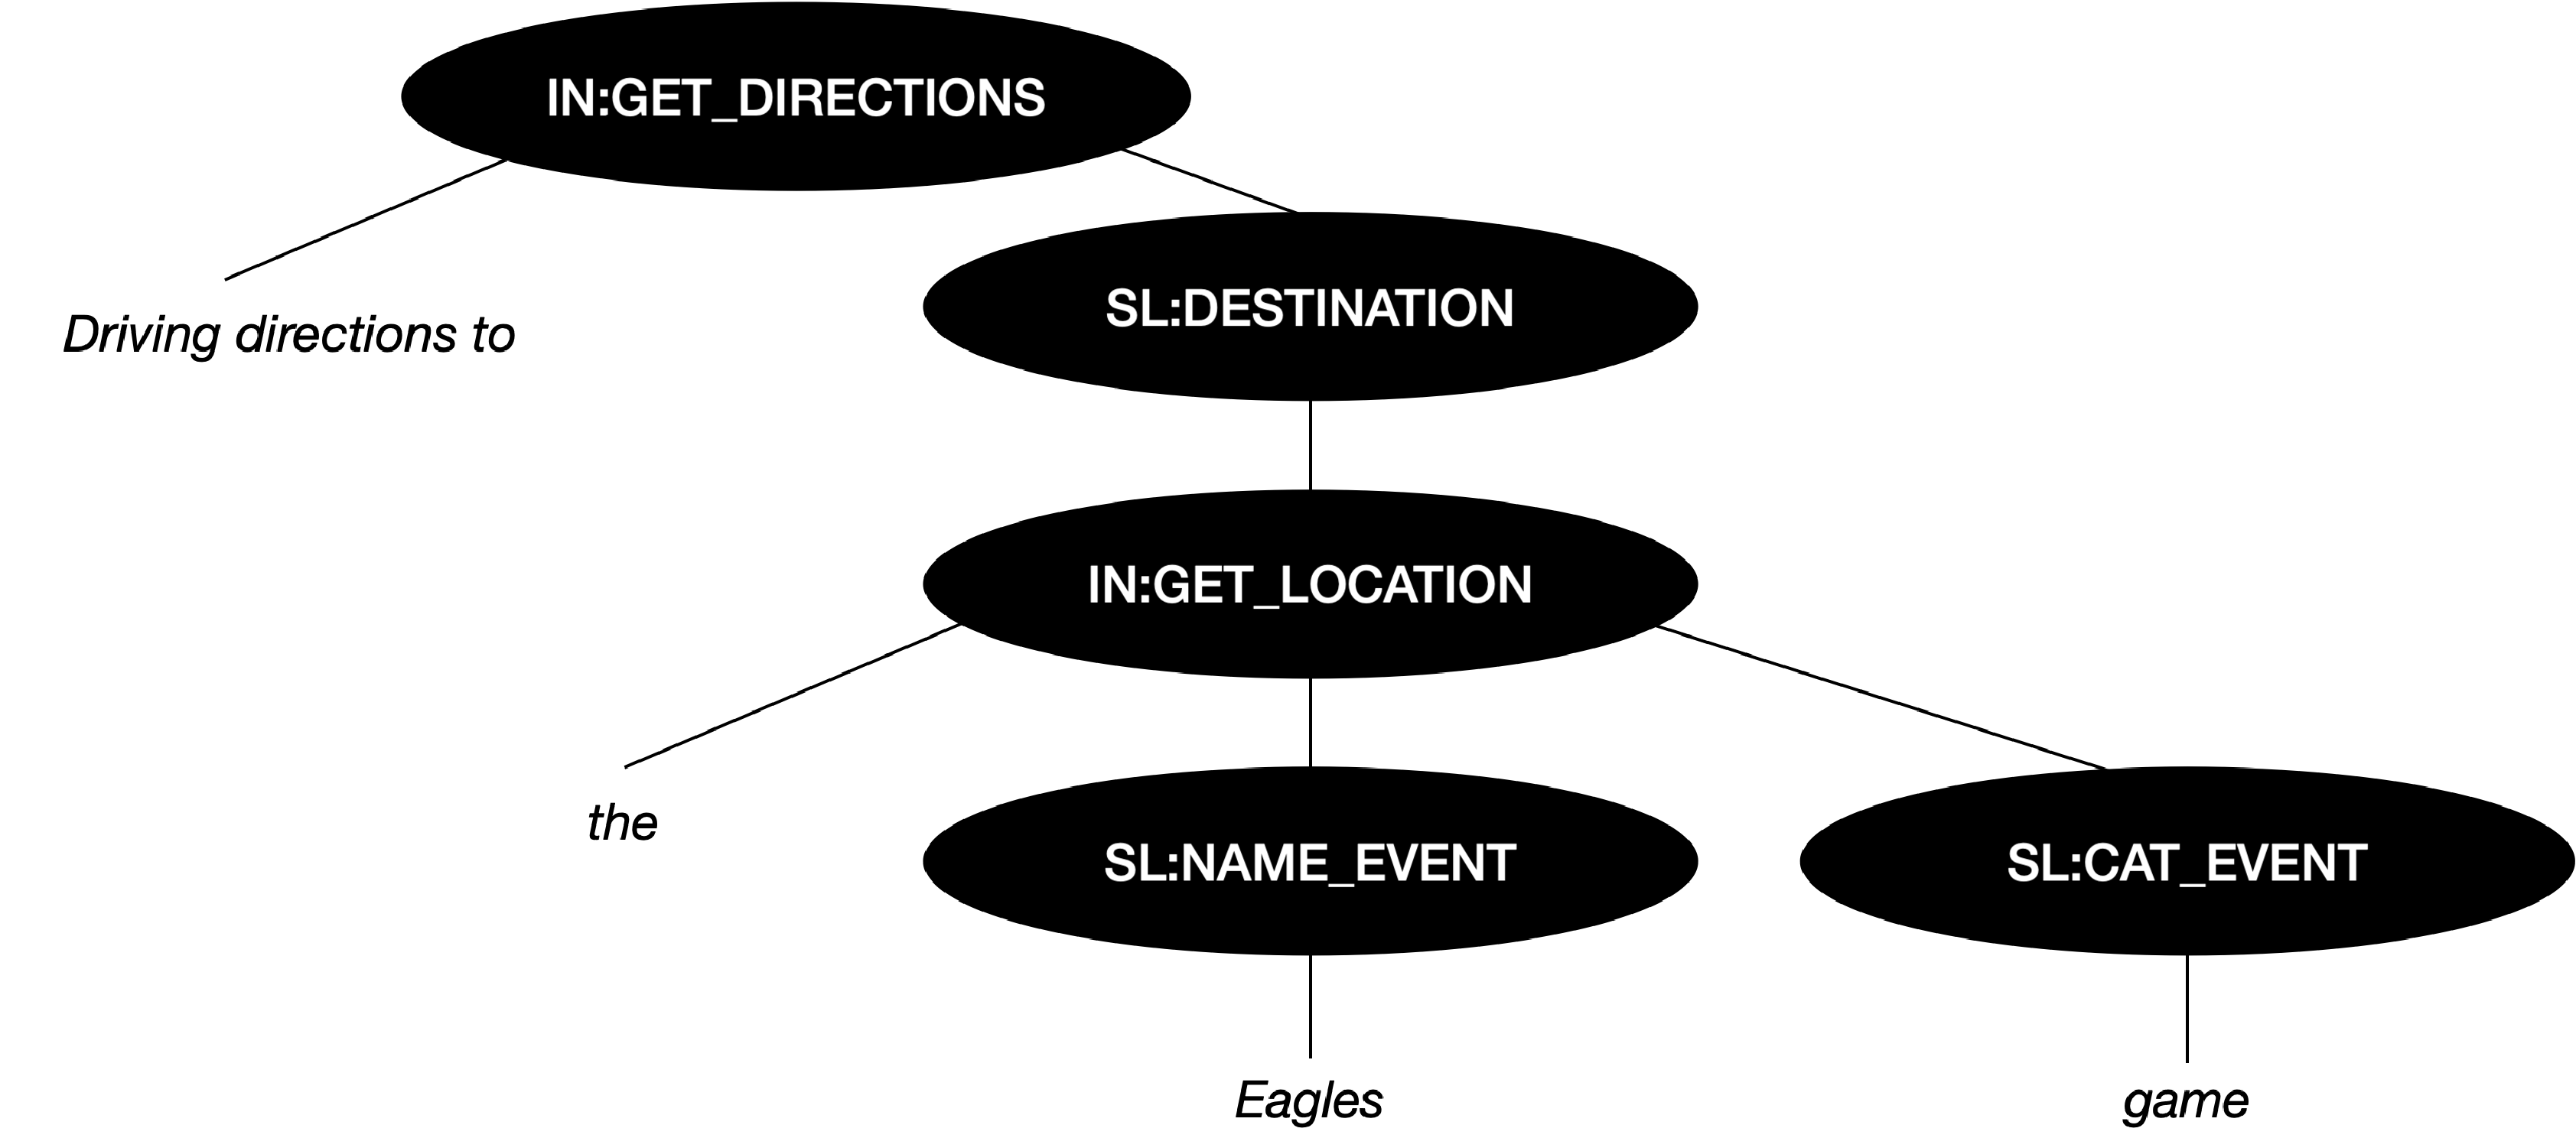
\includegraphics[width=0.95\textwidth]{top-driving.pdf}
\caption{\label{fig:bg:top} TOP examples for conversational
  semantic parsing~(borrowed from the original
  paper~\citep{gupta-etal-2018-semantic-parsing})}
\end{figure}
Recently, conversational parsing has attracted much attention to
represent the dialogue state in a more compositional way, such as the
the hierarchical tree structure in the Task-Oriented dialogue Parsing
~\cite[TOP,][]{gupta-etal-2018-semantic-parsing,aghajanyan2020conversational},
~\cite[TreeDST,][]{cheng2020conversational}, and
~\cite[Dataflow,][]{andreas2020task}. In summary, those conversation
semantic representation offers richer intent slot compositions, and
support complex conversational linguistic phenomena, such as dialogue
state revision and recovering.

In this dissertation, we study the structures of single sentence
representation TOP for dialogue
representations. \autoref{fig:bg:top} shows two examples of the
nested structures of TOP structures. All intents and slots are
non-terminal nodes, and their labels are prefixed with \kw{IN:} or
\kw{SL:} respectively.

The TOP tree structure shares a lot similaries with consituent tree
shown in~\autoref{fig:intro:dog-tree}. It has the following three structural
constraints.
\begin{inparaenum}[(1)]
\item The top level node must be an intent.
\item An intent can have tokens and/or slots as children
\item A slot can have either tokens or intents as its children.
\end{inparaenum}

\subsubsection{Summary of Application-specific Representations}
\label{ssec:bg:summary-application-rep}
\autoref{tbl:bg:app-rep} summarized the application-specific
representations studied in our dissertation. For the application-specific
representations on dialogue, we first introduced sentence-level
anchoring representation: dialogue acts, and we show a specific type
of dialogue act for psychotherapy dialogue called MISC. Then we
introduced the frame-based dialog state tracking, and we showed that
intent classification is also sentence-anchoring tasks, while
requested slot and slot filling tasks can be considered as mixed
anchoring. Finally, to resolve the limitations on non-recursive intent
and slot tagging, we briefly introduced a set of conversational
semantic parsing representations. They offer richer intent slot
compositions and support complex conversational linguistic phenomena,
such as dialogue state revision and recovery.  In this dissertation, we
mainly focused on one of the tree-structural conversational dialogue
representation called TOP, which shares the same phrasal anchoring due
to the similar structure with constituent tree.

\begin{table}[ht]
\caption{The summarization of the application-specific representations studied in this dissertation.}
\label{tbl:bg:app-rep}
  \begin{center}
\setlength{\tabcolsep}{4pt}
{\small
\begin{tabular}{c|c|c|c}
  \toprule
  \hline
  & {\bf MISC}               & {\bf Dialogue State Tracking}            & {\bf TOP}            \\ \hline
  Application    & Psychotherapy      & Task Oriented                      & Task Orientied \\
  Structures     & Sequence Labelling & Intent/Requested Slot/Slot Filling & Tree Parsing   \\
  Anchoring Type & Sentential         & Mixed                              & Phrasal        \\
  \hline
  \bottomrule

\end{tabular}}
\end{center}
\label{tbl:bg:app-rep}
\end{table}



%%% Local Variables:
%%% mode: latex
%%% TeX-master: "../../dissertation-main.ltx"
%%% End:

\section[Deep Linguistic Structured Prediction and Independent
Factorization]{Deep Linguistic Structured Prediction and \\Independent
  Factorization}
\label{sec:background:deepsp}

Due to the power of representation learning, deep learning is widely
used to extract sophisticated representations for the inputs in
various NLP tasks. In this dissertation, instead of focusing on a single
task, we systematically study the representation learning challenges
for multiple tasks based on the independent factorization
assumption. In this section, We first introduce the recent advances
in deep structured prediction with respect to representational
formalism~(\autoref{ssec:bg:formalism}) and introduce the independent
factorization with factor graphs. Then we briefly summarize the
progress on representation learning for natural
language~(\autoref{ssec:bg:rep-learning}) and show why the independent
factorization is possible with the contextualized representations.
Finally, we also summarize the recent advances on
inference~(\autoref{ssec:bg:inference}) for linguistic structured prediction.

%In this dissertation, based on the independent factorization, we study the
%generic inductive biases for \textbf{different purposes more than the
%  accuracy on a single task or a single domain}. For example, by
%exploiting the known linguistic knowledge about anchoring, we study
%five \textit{cross-framework} meaning representation parsing with a
%lexical-anchoring parser and a . By defining two complementary
%dialogueue observers to sequentially predict the MISC code for both
%current and future utterance, our model emphasizes both
%\textit{accurate and real-time} assistance to a therapist. We propose
%to represent the output labels with natural language descriptions for
%\textit{zero-shot learning} on unseen labels~(\autoref{chap:sgd}). In our
%dissertation, we show that during the rapid progress of representation
%learning methods, our proposed inductive biases still can outperform
%the standard usage baselines.

\subsection{Formulations of Structural Interdependence}
\label{ssec:bg:formalism}

Structured prediction refers to machine learning models that learn a
target function to predict mulitple interrelated and dependent
outputs. For representing the target function, different formulations
exists. In this section, we mainly review the recent advances of
representations for modeling the structural interdependences.

\subsubsection{Graphical Models}
\label{sssec:bg:graphic-models}
A graphical model is a probabilistic model using a graph to express
the conditional dependence structure between random
variables. Generally, probabilistic graphical models use a graph-based
representation as the foundation for encoding a distribution over a
multidimensional space, which represents a set of independences that
hold in the specific distribution. Two branches of graphical
representations of distributions are commonly used, namely, Bayesian
networks and Markov random fields. Both families encompass the
properties of factorization and independence, but they differ in the
set of independences they can encode and the factorization of the
distribution that they induce.

\subsubsection{Constrained Conditional Models}
\label{sssec:bg:ccm}
Besides the graphical models to declaratively represent the structural
interdependence, constrained conditional
models~\citep[CCM,][]{chang2012structured} are for the same
goals. More specifically, CCM emphasizes augmenting the learning of
conditional models with declarative constraints. It aims to support
constrained decisions in an expressive output space while maintaining
modularity and tractability of training and inference. These
constraints can express either hard restrictions, completely
prohibiting some assignments, or soft limits, penalizing unlikely
assignments. One popular formalism to represent the constraints is to
use an integer linear programming~(ILP), which has been widely used to
constrain learning in many NLP tasks~\citep{roth2007global}. The
declarative linear objective functions, linear constraints, and the
availabilities of the off-the-shelf solvers make this formalism very
easy to use.

\subsubsection{Declarative Constraints in Deep Learning}
\label{sssec:bg:def-constraints}
Recently, to inject known hand-crafted constraints between discrete
variable assignments in the deep neural networks, one fundamental
challange is how to represent the constraints in end-to-end
differentiable ways~\citep{bach2017hinge}. For example,
\citet{li2019augmenting} propose to use differentiable fuzzy logic
operators to augment the neural networks with boolean
logic. \citet{pacheco2021modeling} introduce a declarative Deep
Relational Learning framework~(\DRAIL) integrating neural
representation learners with probabilistic logic. Besides representing
the constraints as logic forms, much recent work also studies
representing constraints with discrete latent variable models, such as
StructVAE for latent tree-structured
variables~\citep{yin2018structvae, corro2019learning}. Our work on
latent alignment models also falls into this category.

\subsubsection{Learning Constraints in Deep Learning}
\label{sssec:bg:learning-constraints}
Besides injecting declarative constraints, recent research also learn
the constraints in end-to-end
ways. \citet[SPEN,][]{belanger2016structured} define energy functions
that can learn the arbitrary dependencies among parts of structured
outputs by relaxing the whole structured outputs into continuous
vectors, Following this, inference network~\citep{tu2018learning} was
proposed to learn the constrained network for inference, which
approximates the cost-augmented inference during training and then
fine-tuning for test-time inference.

\subsubsection{Independent Factorization}
\label{sssec:bg:ind-factorization}
In this dissertation, we mainly use the undirected Markov random fileds to
represent our independent factorization assumptions. As shown
in~\autoref{fig:bg:graphical-model}, each circle represents a
variable, while each rectangle indicates a factor between the input
sentence variable $x$ and each decomposed segments of output
structures $y$. The difference between the left and right figure is in
the alignment variable $a$ in the center. In the left figure, the
shaded circle $a$ means the alignment is explicitly observed after the
decomposition. In the right figure, the alignment variable $a$ is not
observed.

\begin{figure}[!tbp]
\begin{center}
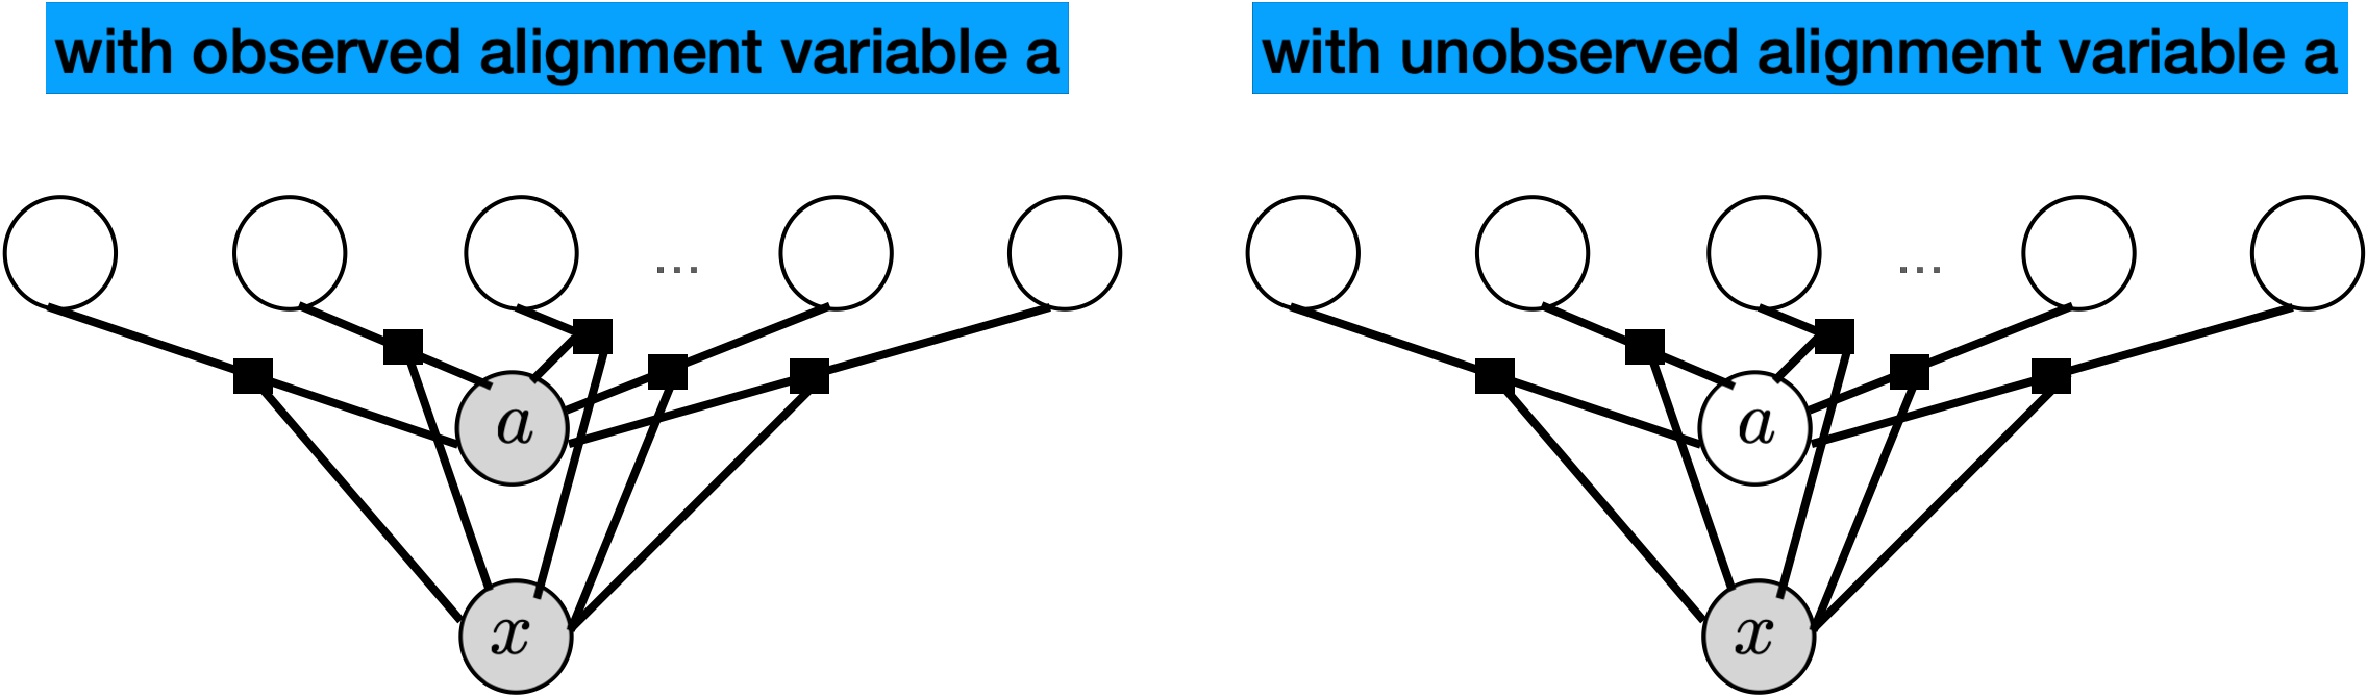
\includegraphics[width=0.90\textwidth]{graphical-models.pdf}
\end{center}
\caption{\label{fig:bg:graphical-model}The factor representation for
  the independent factorization used in our dissertation.}
\end{figure}

As discuessed in \autoref{ssec:intro:bias-dsp}, to apply independent
factorization for each task, we need to resolve three main challenges
to formulate the above factor graph as
$E(x, y) = \sum_{c \in C}E(x, a(y_{c}), y_{c})$, including
\begin{inparaenum}[(1)]
\item \textbf{Output Decomposition:}~Decomposing the output $y$ into a set of independent parts
  $y_{c}$.
\item \textbf{Input Decomposition and Alignments Discovery:}~Decomposing $x$ and derive the aligned input $x_{a_{y_{c}}}$ at
  the index $a_{y_{c}}$.
\item \textbf{Factor Modeling:}~Modelling each $y_{c}$ and its
  relevant parts $x_{a_{y_{c}}}$ to compute the energy score
  $E(x, a(y_{c}), y_{c})$.
\end{inparaenum}

In the following subsection, we show that rapid progress in
contextualized representation learning can offer discriminative
features for modelling the relative parts of $x_{a_{y_{c}}}$, thus
make the challenge~(3)~(factor modeling) of independent factorization possible. Then we
provide the background knowledge about structures in NLP in
\autoref{sec:bg:symbolic}, and we briefly show that such prior
knowledge about anchoring and compositionality are the main source of
inductive biases that guide us to find the decomposition and alignment
in the challenge (1) and (2). We extend the detailed analysis about
independent factorization in each application chapter.

\subsection{Neural Representation Learning}
\label{ssec:bg:rep-learning}

Structured prediction requires the learning can capture both the
discriminative interactions between $x$ and $y$ and also allow
efficient combinatorial optimization over $y$. Ideally, we hope neural
representation learning can handle all of this.

The key challenge of trying to apply analytical and computational
methods to text data are how to represent the text in a way that is
amenable to operations such as similarity, composition, etc. Besides
the early day one-hot representation and TF-IDF
extensions~\citep{jones1972statistical}, word embedding and neural
contextualized representation are widely used in modern deep learning
based models. In this section, we review the recent advances from
static word embedding based methods to attention-based dynamic
features selection and contextualized representation. Finally, we also
introduced the rapid progress in language encoding architectures, from
recurrent neural networks to transformer, and the corresponding
pretrained language models ELMo~\citep{Peters:2018},
BERT~\citep{devlin2019bert}, GPT3~\cite{brown2020language}, etc.

\subsubsection{Static Word Embedding}
\label{sssec:bg:static-embedding}
Word embeddings are commonly categorized into two
types~\citep{Baroni:2014,pennington2014glove,li2015generative},
depending upon the strategies used to induce them:
\begin{inparaenum}[(1)]
\item Prediction-based models, via local data in sentence~(a word'
  context).
\item Count-based models, via the global corpus-wide statistics~(such
  as word counts, co-occurrece).
\end{inparaenum}

Skip-gram with negative sampling~\cite[SGNS,][]{mikolov13w2v} and
GloVe~\cite{pennington2014glove} are among the best-known models for
the two types, respectively. However, they create a single fixed
representation for each word, a notable problem with the static word
embeddings are that all senses of a polysemous word must share a single
vector.

\subsubsection{Contextualized Representation}
\label{sssec:bg:contextualizing}
To resolve the above issue of static word embedding, sequence
encoders, such as LSTM~\citep{hochreiter97lstm},
Transformer~\citep{NIPS2017_7181}, can be used as contextualizing
models to encode the whole context and produce a \kw{contexualized
  representation} for each word, phrase or the whole sentence. In this
way, the contextualized representation dynamically depends on the
entire sentence. Furthermore, based on the neural sequence encoding
architectures, pretraining language models with a large amount of text
can create a more powerful contextualized
representations~\citep{ethayarajh2019contextual}. ELMo~\cite{Peters:2018}
creates contextualized representations of each token by concatenating
the internal states of a 2-layer BiLSTM trained on a bidirectional
language modeling task. In contrast, BERT~\citep{devlin2019bert} and
GPT-2~\citep{radford2018improving} are bidirectional and
unidirectional transformer-based language models,
respectively. \citet{peters2019tune} shows that ELMo contextualized
representation is more suitable to be used as a fixed word embedding,
as also shown in our dissertation on lexical and phrasal anchoring
based parsing~(\autoref{chap:lexical-phrasal}) and sentenctial
anchoring based MISC code prediction~(\autoref{chap:snt}). While for
BERT and GPT-2, finetuning them on downstream task will lead to better
performance, which also inspired us on exploiting natural language
description to understand each output components~(such as intent, slot
labels)~in task-oriented dialogue~(\autoref{chap:sgd}).  One
assumption behind the independent factorization is that local models
with rich features may perform competitively or better than global
models also exists in the pre deep-learning era. Before the rising of deep
learning in 2012, the well known MEMM-based Stanford pos tagger is the
state-of-art model at that time. Instead of using a single normalized,
global CRF model for the sequence modeling, richer features seem
diminish the label biases problems in the
MEMM~\citep{toutanvoa2000enriching,toutanova2003feature}. However, the
rich global features required heavy engineering in ten years ago.
Recently, according to the NLP-Progress
website,~\footnote{\url{http://nlpprogress.com/english/named_entity_recognition.html}
  visited on July 19, 2022}~which tracks the state-of-art models for
each task, we found that the state-of-art models for many sequences
tagging tasks~(such as named entity recognization, part-of-speech
tagging) are attention-based models without any CRF layer. In this
dissertation, the contextualized representation learned from deep
learning is the key to our independent factorization, which helps our
decomposed factor models to make local decisions with a set of
discriminative and global features, without any heavy feature
engineering. Furthermore, large pretrained language model also offers
great power to use natural language in our modeling, such as
prompt-based models~\citep{shin2020autoprompt,liu2021pre}.

\subsection{Inference}
\label{ssec:bg:inference}

Learning with structured data typically involves searching or summing
over a set with an exponential number of structured elements, for
example, the set of all parse trees for a given sentence. In the deep
learning community, it is common to fit models by computing point
estimates, such as the MLE or MAP estimate. Such MAP inference
approaches seem particularly appealing since they are computationally
fairly cheap and can use the before reducing overfitting. In this
way, the neural models only learn a single set of parameters. However,
the point estimation does not capture the associated
uncertainties~\citep{murphy2022probabilistic,wilson2020bayesian}.
Hence, we care about both MAP
and marginal inference in structured prediction research.

\subsubsection{MAP Inference}
\label{sssec:bg:map-inference}
Various exact inference methods are proposed
for MAP inference in NLP tasks. Exact inference methods include
dynamic programming based methods~(such as
viterbi~\citep{viterbi1967error} for hidden markov models, CKY for
context-tree
grammars~\citep{kasami1966efficient,younger1967recognition,cocke1969programming}
, Max Spanning Arborescence for spanning
tree~\citep{chu1965shortest,edmonds1967optimum}, and so on), and
Integer Linear
Programming~\citep{roth2005integer,roth2007global,berant2014modeling}. On the other side, approximate inference methods include various
sampling methods~\citep{finkel2005incorporating,singh2012monte},
search-based
methods~\citep{daume2009search,ross2011reduction,chang2015learning},
and Linear Programming
Relaxations~\citep{rush2012tutorial,werner2014power}.

\subsubsection{Marginal Inference}
\label{sssec:bg:marginal-inference}
Integration is at the heart of marginal inference, whereas
differentiation is at the heart of optimization. Corresponding to the
each of the above exact MAP inference algorithms, various methods are
proposed for marginal inference. They compute marginal probabilities
and partition functions which are central to many methods, such as
EM~\citep{baker1979trainable,weizenbaum1966eliza}, constrative
estimation~\citep{smith2005contrastive}, Conditional Random
Field~\citep[CRF,][]{lafferty01crf}, max-margin training over all
candidate targets~\citep{koller2004max}. For linguistic structured
prediction, exact marginal inference methods include forward-backward
algorithm for HMM~\citep{binder1997space},
Inside-outside~\citep{baker1979trainable}, Matrix-Tree Theorem for
nonprojective dependency
structures~\citep{koo-etal-2007-structured,liu2018learning}.

In this dissertation, we use variational inference to marginalize out the
latent alignment variable
in~\autoref{ssec:lex-phr:latent-alignment}. While for the other parts
of this dissertation, the assumption of independent factorization simplified
the inference into either greedy~(\autoref{chap:snt} and
\autoref{chap:sgd}) or dynamic programming based exact MAP
inference~(such as the dynamic programming parsing the dependency and
constituency structures in~\autoref{ssec:lex-phr:two-stage} and
~\autoref{sec:lex-phr:cky-based}, respectively)

%%% Local Variables:
%%% mode: latex
%%% TeX-master: "../../dissertation-main.ltx"
%%% End:


\section{Chapter Summary}
\label{sec:bg:summary}
In this chapter, we first summarized the recent advances in deep
structured prediction for representational formalism,
learning and inference, respectively. For representational formalism,
we introduce graphic model to represent the structural
interdependence, and represent the main assumption of the independent
factorization as two factor graphs
in~\autoref{fig:bg:graphical-model}. Then we overviewed the
development of representation learning methods for natural language,
from feature selection to deep learning based on contextualized
representation learning methods. We also reviewed the recent advances
of MAP inference and Marginal Inference in deep learning.

The second part of this section introduces the background of symbolic
representation for natural language, including the broad-coverage
meaning representations and application-specific
representations. Instead of studying structured prediction for each
linguistic structured prediction tasks separately, based on
independent factorization, we firstly categorize those symbolic
representations according to the anchoring types, summarized
in~\autoref{ssec:bg:summary-broad-coverage}
and~\autoref{ssec:bg:summary-application-rep}. Then based on the
background, in the following chapters, we study the detailed
strategies for independent factorization by exploiting the structural
inductive biases and natural language as inductive biases.

%%% Local Variables:
%%% mode: latex
%%% TeX-master: "../../thesis-main.ltx"
%%% End:


\index{gnu}

\index{gnu!diet}
\index{gnu!diet!wet season}
\index{gnu!diet!dry season}

\index{rhinodon}
\index{rhinodont}
\index{rhinoceros}
\index{rhinoceros horn}
\index{rhinocerite}
\index{rhinestone}
\index{Rhineland}
\index{Rhinegrave}
\index{Rhine berry}
\index{rhea}
\index{rat}
\index{raccoon}
\index{Queensland viper}
\index{quail}
\index{quagga}
\index{puffin}
\index{pterodactyl}
\index{pronghorn (\bioname{Antilocapra americana})}
\index{peccary}
\index{panther}
\index{panda}
\index{opossum}
\index{okapi}
\index{octopus}
\index{ocelot (\bioname{Leopardus pardalis})}
\index{nilgai}
\index{Neanderthal}
\index{nautilus}
\index{narwhal}
\index{muskrat}
\index{musk ox}
\index{moose (\bioname{Alces alces})}
\index{mastodon}
\index{mastiff}
\index{marmot (\bioname{Marmota marmota})}
\index{margay (\bioname{Leopardus wiedii})}
\index{manatee (\bioname{Trichechus inunguis})}
\index{mammoth}

\index{Alces alces@\bioname{Alces alces}}
\index{Antilocapra americana@\bioname{Antilocapra americana}}
\index{Marmota marmota@\bioname{Marmota marmota}}

%%% Local Variables:
%%% mode: latex
%%% TeX-master: "../thesis-main.ltx"
%%% End:
